\documentclass[10pt,a4paper]{article}

% ---------------------------------------------------------------- packages
\usepackage[T1]{fontenc}
\usepackage[utf8]{inputenc}
\usepackage[semibold]{XCharter}
\usepackage[scaled=0.82]{beramono}
\usepackage[scaled=0.90]{helvet}
\usepackage{microtype}
\usepackage[margin=2.3cm,headheight=14pt]{geometry}
\usepackage{graphicx}
\usepackage{booktabs}
\usepackage{tikz}
\usetikzlibrary{arrows.meta,positioning,fit,calc,shapes.misc}
\usepackage{listings}
\usepackage{xcolor}
\usepackage[most]{tcolorbox}
\usepackage{titlesec}
\usepackage{enumitem}
\usepackage{fancyhdr}
\usepackage[colorlinks=true,linkcolor=linkblue,urlcolor=linkblue]{hyperref}

% ---------------------------------------------------------------- colors
\definecolor{linkblue}{HTML}{1a5276}
\definecolor{codebg}{HTML}{F6F6F4}
\definecolor{codeframe}{HTML}{D8D8D2}
\definecolor{kwcolor}{HTML}{7A2E8E}
\definecolor{strcolor}{HTML}{1B7A3D}
\definecolor{cmtcolor}{HTML}{8A8A85}
\definecolor{boxblue}{HTML}{EAF1F7}
\definecolor{boxblueframe}{HTML}{9DB8CE}
\definecolor{corecol}{HTML}{DCE8F5}
\definecolor{qtcol}{HTML}{E4F2E0}
\definecolor{edcol}{HTML}{FBEEDB}
\definecolor{pkgcol}{HTML}{F5E3E3}

% ---------------------------------------------------------------- listings
\lstdefinestyle{py}{
  language=Python,
  basicstyle=\ttfamily\small,
  keywordstyle=\color{kwcolor}\bfseries,
  stringstyle=\color{strcolor},
  commentstyle=\color{cmtcolor}\itshape,
  showstringspaces=false,
  backgroundcolor=\color{codebg},
  frame=single, rulecolor=\color{codeframe}, framerule=0.4pt,
  xleftmargin=8pt, xrightmargin=4pt, framexleftmargin=6pt,
  aboveskip=8pt, belowskip=8pt,
  breaklines=true,
  columns=fullflexible, keepspaces=true,
}
\lstset{style=py}
\newcommand{\code}[1]{\texttt{\small #1}}

% ---------------------------------------------------------------- callout box
\newtcolorbox{scfnote}{%
  colback=boxblue, colframe=boxblueframe, boxrule=0.5pt, arc=1.5pt,
  left=7pt, right=7pt, top=5pt, bottom=5pt,
  before skip=10pt, after skip=10pt,
  title={\sffamily\bfseries\small Visual-SCF note},
  fonttitle=\color{black},
  coltitle=black, attach title to upper={\par\smallskip}}

% ---------------------------------------------------------------- headings
\titleformat{\section}{\Large\sffamily\bfseries}{\thesection}{0.8em}{}
\titleformat{\subsection}{\large\sffamily\bfseries}{\thesubsection}{0.8em}{}
\titleformat{\subsubsection}{\normalsize\sffamily\bfseries}{\thesubsubsection}{0.8em}{}
\titlespacing*{\section}{0pt}{18pt}{6pt}
\titlespacing*{\subsection}{0pt}{12pt}{4pt}

\setlist{itemsep=2pt, topsep=4pt}

\pagestyle{fancy}
\fancyhf{}
\fancyhead[L]{\sffamily\small Ryven internals}
\fancyhead[R]{\sffamily\small\thepage}
\renewcommand{\headrulewidth}{0.3pt}

\setlength{\parindent}{0pt}
\setlength{\parskip}{5pt}

% ================================================================== document
\begin{document}

\begin{titlepage}
\centering
\vspace*{3cm}
{\Huge\sffamily\bfseries How Ryven Works Internally\par}
\vspace{0.8cm}
{\Large A tour of ryvencore, ryvencore-qt, and the Ryven editor\par}
\vspace{0.4cm}
{\large --- written for the Visual-SCF project ---\par}
\vspace{2cm}
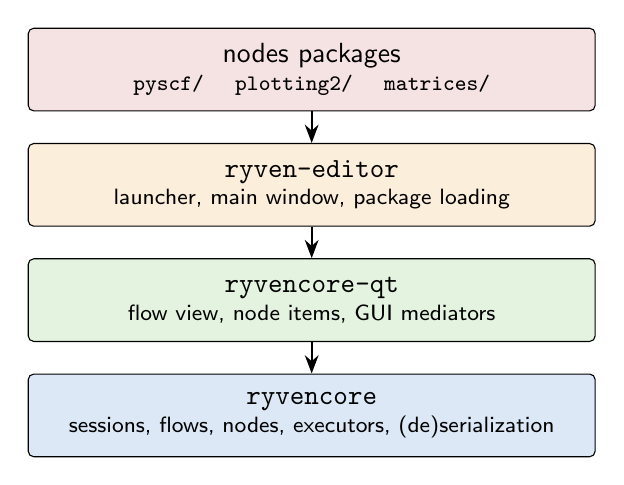
\begin{tikzpicture}[
  layer/.style={draw, rounded corners=2pt, minimum width=7.2cm, minimum height=1.05cm,
                font=\sffamily, align=center},
  note/.style={font=\sffamily\footnotesize\itshape, text=black!60, align=left}]
  \node[layer, fill=pkgcol]  (pkg)  {nodes packages\\[-2pt]{\footnotesize \texttt{pyscf/} \quad \texttt{plotting2/} \quad \texttt{matrices/}}};
  \node[layer, fill=edcol,  below=4mm of pkg]  (ed)   {\texttt{ryven-editor}\\[-2pt]{\footnotesize launcher, main window, package loading}};
  \node[layer, fill=qtcol,  below=4mm of ed]   (qt)   {\texttt{ryvencore-qt}\\[-2pt]{\footnotesize flow view, node items, GUI mediators}};
  \node[layer, fill=corecol,below=4mm of qt]   (core) {\texttt{ryvencore}\\[-2pt]{\footnotesize sessions, flows, nodes, executors, (de)serialization}};
  \draw[-{Stealth}, thick] (pkg) -- (ed);
  \draw[-{Stealth}, thick] (ed) -- (qt);
  \draw[-{Stealth}, thick] (qt) -- (core);
\end{tikzpicture}
\vspace{2cm}

{\small Based on the checkouts at \texttt{\~{}/Projects/Ryven} (fork of Ryven 3.5) and\\
\texttt{\~{}/Projects/ryvencore} (v0.5.0), as installed editable into Visual-SCF's venv.\par}
\vfill
{\small July 2026\par}
\end{titlepage}

\tableofcontents
\newpage

% ==================================================================
\section{The big picture}

Ryven is not one program but a stack of three Python packages, deliberately split so that
the graph engine has no GUI dependency at all:

\begin{itemize}
\item \textbf{ryvencore} --- the headless flow engine. It knows about sessions, flows
      (graphs), nodes, ports, connections, data wrappers, execution algorithms, add-ons,
      and how to serialize all of it to a JSON-compatible dict. It never imports Qt.
      Lives in its own repository (\code{\textasciitilde/Projects/ryvencore}).
\item \textbf{ryvencore-qt} --- the Qt frontend for ryvencore. It wraps a core
      \code{Session} in a \code{SessionGUI}, renders each \code{Flow} as a
      \code{QGraphicsScene}-based \code{FlowView}, and mediates between abstract nodes
      and their visual items. Lives in the Ryven monorepo
      (\code{Ryven/ryvencore-qt}).
\item \textbf{ryven-editor} --- the application: command-line parsing, the startup
      dialog, the main window, the nodes-package import system
      (\code{ryven.node\_env} / \code{ryven.gui\_env}), themes, the built-in console,
      and the code editor. Lives in \code{Ryven/ryven-editor}.
\end{itemize}

A \emph{nodes package} such as Visual-SCF's \code{pyscf/} sits on top of all three: its
\code{nodes.py} imports only from \code{ryven.node\_env} (which re-exports ryvencore
types), while its \code{gui.py} imports from \code{ryven.gui\_env} (which re-exports
ryvencore-qt widget classes). This split is what makes node logic importable in headless
contexts.

The key mental model for everything that follows:

\begin{center}
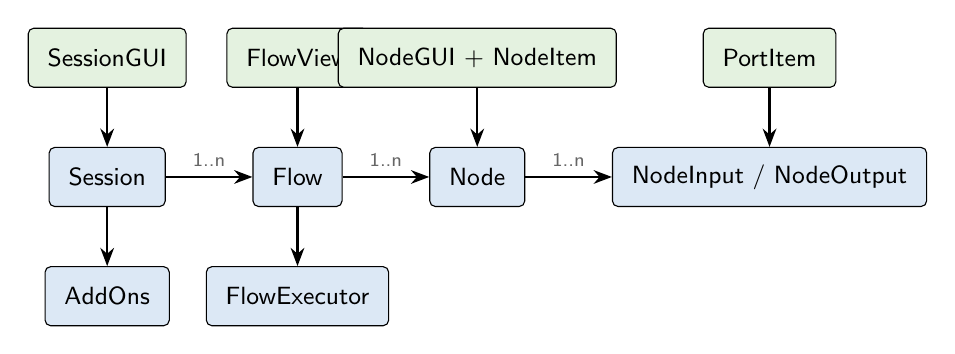
\begin{tikzpicture}[
  obj/.style={draw, rounded corners=2pt, fill=corecol, font=\sffamily\small,
              minimum height=0.75cm, inner xsep=7pt},
  gobj/.style={draw, rounded corners=2pt, fill=qtcol, font=\sffamily\small,
              minimum height=0.75cm, inner xsep=7pt},
  lbl/.style={font=\sffamily\scriptsize, text=black!60},
  arr/.style={-{Stealth}, thick}]
  \node[obj] (sess) {Session};
  \node[obj, right=1.1cm of sess] (flow) {Flow};
  \node[obj, right=1.1cm of flow] (node) {Node};
  \node[obj, right=1.1cm of node] (port) {NodeInput / NodeOutput};
  \node[obj, below=0.75cm of flow] (exec) {FlowExecutor};
  \node[obj, below=0.75cm of sess] (addon) {AddOns};
  \node[gobj, above=0.75cm of sess] (sgui) {SessionGUI};
  \node[gobj, above=0.75cm of flow] (fview) {FlowView};
  \node[gobj, above=0.75cm of node] (ngui) {NodeGUI + NodeItem};
  \node[gobj, above=0.75cm of port] (pitem) {PortItem};
  \draw[arr] (sess) -- node[lbl,above]{1..n} (flow);
  \draw[arr] (flow) -- node[lbl,above]{1..n} (node);
  \draw[arr] (node) -- node[lbl,above]{1..n} (port);
  \draw[arr] (flow) -- (exec);
  \draw[arr] (sess) -- (addon);
  \draw[arr] (sgui) -- (sess);
  \draw[arr] (fview) -- (flow);
  \draw[arr] (ngui) -- (node);
  \draw[arr] (pitem) -- (port);
\end{tikzpicture}
\end{center}

The bottom row (blue) is pure ryvencore and works without a display. The top row (green)
is ryvencore-qt: each GUI object holds a reference to the core object it represents,
subscribes to its events, and adds a Qt item to the scene. The core never calls into the
GUI directly --- it emits events; whether anything listens is the frontend's business.

% ==================================================================
\section{ryvencore: the object model}

\subsection{\texttt{Base}: identity, events, and the serialization hook}

Almost every core class (\code{Session}, \code{Flow}, \code{Node}, \code{NodePort},
\code{Data}) derives from \code{Base} (\code{ryvencore/Base.py}), which provides three
things:

\textbf{Global IDs.} Every object gets a \code{global\_id} from a process-wide counter.
When an object is loaded from a save file, its old ID is remembered as
\code{prev\_global\_id} and registered in a static map, so components that stored
references by ID (notably GUI state) can re-associate after load. (The map is never
pruned --- a known, commented, benign leak.)

\textbf{A tiny pub/sub system.} \code{Event} is a minimal observer implementation:
\code{sub(callback, nice=0)}, \code{unsub()}, \code{emit(*args)}. The \code{nice}
value orders callbacks (lower fires first); internal wiring such as flow bookkeeping
subscribes at \code{nice=-5} so it runs before user-visible handlers. This is the
mechanism behind \code{flow.node\_added}, \code{node.updating},
\code{node.update\_error}, etc. --- and ryvencore-qt's whole job is translating these
into Qt signals.

\textbf{The \code{complete\_data} hook.} Serialization is initiated by the core
(\code{data()} methods returning dicts), but the frontend can register a single static
function, \code{Base.complete\_data\_function}, which is applied to serialized dicts to
\emph{supplement} them with GUI-only state. This is how node positions and widget state
end up inside a project file without the core knowing they exist
(section~\ref{sec:serialization}).

\subsection{\texttt{Session}}

\code{Session} (\code{ryvencore/Session.py}) is the project root. It owns:

\begin{itemize}
\item \code{flows} --- the list of \code{Flow} objects (a Ryven project can have several
      tabs, each is a flow);
\item \code{nodes} --- a \emph{set of node classes} registered via
      \code{register\_node\_type()}; only registered classes may be instantiated in
      flows, and loading a project resolves node identifiers against this set;
\item \code{data\_types} --- registered \code{Data} subclasses, keyed by identifier
      (needed to reconstruct typed payloads on load);
\item \code{addons} --- add-on singletons discovered from
      \code{ryvencore/addons/*.py} (Variables, Logging) when constructed with
      \code{load\_addons=True}.
\end{itemize}

\code{Session.load(data)} restores add-ons first, then recreates each flow. It contains
backward-compatibility shims (older projects stored flows under a \code{scripts} key).

\subsection{\texttt{Flow}: the graph}

\code{Flow} (\code{ryvencore/Flow.py}) manages nodes and edges. A flow is a directed
multigraph where the vertices are \emph{ports}, not nodes. Three data structures matter:

\begin{lstlisting}
self.nodes:            List[Node]
self.graph_adj:        Dict[NodeOutput, List[NodeInput]]   # out -> fan-out
self.graph_adj_rev:    Dict[NodeInput, Optional[NodeOutput]] # in -> 0 or 1 source
self.node_successors:  Dict[Node, List[Node]]              # for executors
\end{lstlisting}

The cardinality is asymmetric by design: an output may feed any number of inputs, but an
input has \emph{at most one} incoming connection. \code{connected\_output(inp)} therefore
returns a single port or \code{None}, which is why node code can treat ``my input's
value'' as a scalar lookup.

\code{create\_node(cls, data=None)} instantiates the class with the tuple
\code{(flow, session)} --- this is the mysterious \code{params} argument every node's
\code{\_\_init\_\_} forwards to \code{super()}. It then wires port-change events,
calls \code{node.initialize()} (which builds ports from \code{init\_inputs} /
\code{init\_outputs}, or from saved data when loading), optionally calls
\code{node.load(data)}, and finally places the node (\code{place\_event()} fires).

\code{connect\_nodes(out, inp)} validates the request (no self-connections, matching
port types, correct directions), updates the adjacency maps, and then calls
\code{executor.conn\_added(out, inp, silent=...)}. In the default executor,
\textbf{a new connection immediately triggers an update on the receiving node} ---
unless \code{silent=True}, which is exactly what project loading uses to avoid an update
storm while rebuilding a saved graph.

\subsection{\texttt{Node} and its ports}

\code{Node} (\code{ryvencore/Node.py}) is the base for all node blueprints.
Class attributes describe the blueprint (\code{title}, \code{tags}, \code{version},
\code{init\_inputs}, \code{init\_outputs}, \code{identifier});
instances hold live ports and state. The three methods that make up the
\emph{data-plane API} all delegate to the flow's executor:

\begin{lstlisting}
def update(self, inp=-1):            # request own update_event
    self.updating.emit(inp)
    self.flow.executor.update_node(self, inp)

def input(self, index) -> Optional[Data]:
    return self.flow.executor.input(self, index)

def set_output_val(self, index, data):
    assert isinstance(data, Data)    # payloads MUST be wrapped
    self.flow.executor.set_output_val(self, index, data)
\end{lstlisting}

That \code{assert} is why every Visual-SCF node wraps results in \code{Data(...)}
(or a subclass) before emitting.

The \emph{virtual methods} a node implementation may override form its life cycle:

\begin{center}
\small
\begin{tabular}{@{}lll@{}}
\toprule
\textbf{Method} & \textbf{Called when} & \textbf{Typical use}\\
\midrule
\code{update\_event(inp)} & an input fired, or \code{update()} & the node's computation\\
\code{place\_event()}     & node added to flow (before edges)  & timers, addon access\\
\code{remove\_event()}    & node removed                       & stop threads/timers\\
\code{get\_state()}       & saving                             & return JSON-able dict\\
\code{set\_state(d, v)}   & loading (before edges)             & restore fields\\
\code{rebuilt()}          & loading, \emph{after} edges exist  & re-fire computation\\
\bottomrule
\end{tabular}
\end{center}

Ports are thin: \code{NodeOutput} holds \code{val} (the current \code{Data}),
\code{NodeInput} holds an optional \code{default}. There is no queueing and no
copying --- an input ``having a value'' literally means \emph{the output it is connected
to has a non-\code{None} \code{val}}.

\subsection{\texttt{Data}: the payload envelope}

\code{Data} (\code{ryvencore/Data.py}) wraps whatever a node emits in an object with a
\code{payload} property plus serialization support (pickle by default). Two properties
of the design are worth internalizing:

\begin{itemize}
\item \textbf{Payloads are shared, not copied.} If one output feeds two consumers and
      the first mutates the payload in place, the second sees the mutation. Subclasses
      can override the \code{payload} property to return copies if isolation matters.
\item \textbf{Custom subclasses must be registered.} On load, output values are
      reconstructed by looking up the data-type identifier in
      \code{session.data\_types}; unregistered types are skipped with an error. Ryven's
      \code{export\_nodes(..., data\_types=[...])} handles registration for package
      types like \code{MatrixData}.
\end{itemize}

\begin{scfnote}
Visual-SCF relies on the sharing behavior implicitly: a PySCF \code{Mole} object
flows by reference from \code{MolNode} to every consumer. Nothing mutates it
downstream, so this is safe --- but it is a convention, not something the framework
enforces. The \code{hasattr(self.input(i), 'payload')} guard used throughout
\code{inputs\_ready()} works because \code{Node.input()} returns \code{None} when the
connected output has never been set (and \code{None} has no \code{payload} attribute).
\end{scfnote}

% ==================================================================
\section{Flow execution: the executors}
\label{sec:executors}

Execution semantics are pluggable. \code{Flow} holds an executor object, selected by the
flow's \emph{algorithm mode} (persisted in the project file); \code{Node.update()},
\code{Node.input()}, \code{Node.set\_output\_val()} and \code{Node.exec\_output()} are
all forwarded to it. Three algorithms exist in
\code{ryvencore/FlowExecutor.py}:

\subsection{\texttt{DataFlowNaive} (the default)}

The default mode (\code{FlowAlg.DATA}) is a synchronous push model.
Setting an output propagates \emph{immediately and recursively}:

\begin{lstlisting}
# Node.set_output_val() =>
def set_output_val(self, node, index, data):
    out = node.outputs[index]
    out.val = data
    for inp in self.graph[out]:
        inp.node.update(inp=inp.node.inputs.index(inp))
\end{lstlisting}

So a call to \code{set\_output\_val} inside node $A$'s \code{update\_event} runs node
$B$'s \code{update\_event} \emph{before $A$'s has returned} --- flow execution is plain
Python call-stack recursion, on the Qt main thread, with no scheduling, no deferral,
and no cycle detection. Consequences:

\begin{itemize}
\item \textbf{Order:} with multiple outgoing edges, activation order is the list order
      of \code{graph\_adj[out]} (i.e.\ connection creation order), but is documented as
      undefined --- do not rely on it.
\item \textbf{Diamonds are expensive:} if $A$ feeds $B$ and $C$, which both feed $D$,
      then one update of $A$ updates $D$ twice; nested diamonds grow exponentially.
\item \textbf{Cycles do not terminate:} a feedback edge means infinite recursion until
      Python's recursion limit kills it. The engine \emph{assumes} no non-terminating
      feedback loops; breaking a cycle is the node author's job.
\item \textbf{Exceptions are contained:} \code{update\_node} wraps
      \code{update\_event} in \code{try/except}; failures go to
      \code{node.update\_err(e)}, which emits the \code{update\_error} event (shown by
      the GUI as a red indicator bubble on the node item) rather than unwinding the
      whole propagation.
\item \textbf{New connections fire immediately:} \code{conn\_added} updates the
      receiving node right away (except during silent/loading operations). A node must
      therefore tolerate being updated when only some of its inputs are connected ---
      this is the entire reason for the \code{inputs\_ready()} idiom.
\end{itemize}

\begin{scfnote}
The SCF feedback loop (\code{SCFStepNode}) exists precisely because of the naive
executor's cycle behavior. The graph
\code{SCF Step} $\to$ \code{Fock} $\to$ \code{Get MO Coeff} $\to$ \code{Make 1-RDM}
$\to$ \code{SCF Step} is a true cycle; if \code{SCFStepNode.update\_event} propagated
on arrival of ``New 1-RDM'', \code{set\_output\_val} would recurse forever.
Instead the node absorbs that input silently and only re-emits when the user clicks
\emph{Step} --- turning the runaway recursion into one user-paced lap around the loop
per click. Each click still executes the whole chain synchronously before returning
to the Qt event loop.
\end{scfnote}

\subsection{\texttt{DataFlowOptimized}}

An alternative mode (\code{FlowAlg.DATA\_OPT}) that guarantees each connection activates
\emph{at most once per execution}. When an execution starts (some node or output is
updated from outside), it runs a BFS/DP pass over the successor component to count, for
every node, how many incoming connections could still deliver data
(\code{generate\_waiting\_count}). Outputs written during the execution are buffered
(\code{out.val} is set, but successors are not updated); a node's outputs are propagated
only when its waiting count reaches zero, i.e.\ when no predecessor can still change its
inputs. The DP table is cached between executions while the graph is unchanged
(\code{flow\_changed} flag maintained by \code{Flow}).

This fixes the diamond blow-up, but tightens the assumptions: the graph must be acyclic
and nodes must not modify their ports during execution. It would \emph{not} be safe for
Visual-SCF's cyclic SCF graph.

\subsection{\texttt{ExecFlowNaive}}

The third mode (\code{FlowAlg.EXEC}) implements UnrealEngine-blueprint-style execution
with dedicated \code{exec}-type ports: triggers travel forward along exec connections
(\code{exec\_output()}), while data is \emph{pulled backward on demand} --- when an
updating node calls \code{self.input(i)} and the connected predecessor has not yet
updated in this execution, the predecessor's \code{update\_event(-1)} is invoked first
so it can push a fresh value. Ryven exposes the mode per flow, but Visual-SCF uses pure
data flows only.

% ==================================================================
\section{The nodes package system}

\subsection{Anatomy and import mechanics}

A nodes package is a directory containing a \code{nodes.py} (mandatory) and usually a
\code{gui.py}. It is identified by its \emph{directory basename} --- which is why the
project's package is called \code{pyscf} and why that name collides gracefully with the
\code{pyscf} library only because Ryven loads the file by path, not via
\code{import}.

Loading happens in \code{ryven/main/packages/nodes\_package.py::import\_nodes\_package()}:

\begin{enumerate}
\item The environment variable \code{RYVEN\_MODE} must be set (\code{'gui'} or
      \code{'no-gui'}); the editor sets it in \code{Ryven.py} before any package import.
\item \code{NodesEnvRegistry.current\_package} is set to the package being imported ---
      global state consumed by \code{export\_nodes()}.
\item \code{nodes.py} is executed via \code{load\_from\_file()}
      (\code{importlib} machinery, no package installation involved).
\item If in GUI mode, all functions registered with \code{@on\_gui\_load} are invoked
      (this is when \code{gui.py} gets imported); in headless mode they are skipped
      entirely, so \code{nodes.py} must never import Qt at module level.
\item The registry's accumulated node and data classes are consumed and handed to the
      session for registration.
\end{enumerate}

\subsection{What \texttt{export\_nodes()} actually does}

Beyond collecting classes in the registry, \code{export\_nodes()}
(\code{ryven/main/packages/node\_env.py}) performs identifier surgery on each node
class:

\begin{itemize}
\item builds the identifier as \code{<class name>} if not explicitly set, then
      prefixes it with the package name: the saved-file identifier of
      \code{MolNode} is \code{pyscf.MolNode};
\item appends fallbacks to \code{legacy\_identifiers} so projects saved under older
      naming schemes still resolve;
\item registers exported \code{Data} subclasses under
      \code{<pkg>.<ClassName>} the same way.
\end{itemize}

When a project is loaded, \code{node\_from\_identifier()} resolves each saved
identifier against registered classes, falling back to \code{legacy\_identifiers} ---
this is the entire backward-compatibility story for renamed/moved node classes.

\subsection{Binding GUIs: \texttt{@node\_gui}}

\code{ryven.gui\_env} provides the \code{node\_gui(NodeClass)} decorator, which simply
sets \code{NodeClass.GUI = <NodeGUI subclass>} (with a guard against double
registration). Nothing is instantiated at binding time; the attribute is read later when
a node item is built for a placed node. GUI classes are \emph{inherited} by node
subclasses unless overridden.

% ==================================================================
\section{ryvencore-qt: how the GUI is wired}

\subsection{\texttt{SessionGUI} and \texttt{FlowView}}

\code{SessionGUI} wraps the core session (created with \code{gui=True,
load\_addons=True}), stores itself as \code{session.gui}, and subscribes to
\code{flow\_created} --- so whenever a flow appears (new or loaded), it constructs a
matching \code{FlowView}. It also registers the frontend's
\code{complete\_data} function with ryvencore (see \S\ref{sec:serialization}).

\code{FlowView} is a \code{QGraphicsView}/\code{QGraphicsScene} pair, and is where all
direct user interaction lives: placing nodes (it listens to \code{flow.node\_added} and
creates a \code{NodeItem}), dragging connections between \code{PortItem}s (validated
through \code{flow.check\_connection\_validity} before
\code{flow.connect\_nodes} is called), selection, undo/redo commands
(\code{FlowCommands.py}), zooming, themes (\code{FlowTheme.py}), and the node-list
popup for adding nodes.

\subsection{\texttt{NodeGUI}: the mediator}

For each placed node, the frontend builds a pair of objects:

\begin{itemize}
\item \code{NodeGUI} (\code{ryvencore\_qt/src/flows/nodes/NodeGUI.py}) --- a
      \code{QObject} constructed with \code{(node, session\_gui)}. Its constructor does
      \code{setattr(node, 'gui', self)} --- \textbf{this is where the
      \code{node.gui} attribute comes from}, and why headless nodes must guard with
      \code{hasattr(self, 'gui')}: in no-GUI mode the attribute simply never exists.
      It subscribes to the node's core events (\code{updating},
      \code{update\_error}, ports added/removed) and re-emits them as Qt signals.
      It also owns the \code{actions} dict --- the node's right-click menu ---
      mapping labels to \code{\{'method': callable\}} entries, (de)serialized by
      method \emph{name}.
\item \code{NodeItem} --- the actual \code{QGraphicsItem} in the scene: title label,
      port items, the collapsible body, the error indicator, and the animator. It
      reads the class attributes of the bound \code{NodeGUI} subclass:
      \code{color}, \code{style}, \code{display\_title},
      \code{main\_widget\_class} and \code{main\_widget\_pos}
      (\code{'below ports'} or \code{'between ports'}).
\end{itemize}

If \code{main\_widget\_class} is set, \code{NodeItem} instantiates it, passing
\code{(node, item, node\_gui)} --- the widget's \code{params}. The widget is a normal
\code{QWidget} embedded into the graphics scene through a
\code{QGraphicsProxyWidget} subclass (\code{FlowViewProxyWidget}). Embedding via proxy
is exactly why Visual-SCF's 3D viewer had to become a pure-QPainter widget: native
surfaces (GL/VTK) do not survive inside \code{QGraphicsProxyWidget}.

Main widgets participate in persistence through their own
\code{get\_state()}/\code{set\_state()} pair: \code{NodeItem} pickles the widget state
into the item's data under \code{'main widget data'} on save and restores it on load.
Note the asymmetry with nodes: widget \code{set\_state(data)} takes no version argument.

\subsection{Update flow, end to end}

Putting sections \ref{sec:executors} and this one together, a click on Visual-SCF's
\emph{Step} button travels like this:

\begin{enumerate}[itemsep=1pt]
\item Qt delivers the click to \code{SCFStepWidget}; the handler calls
      \code{self.node.step()} --- widget-to-node communication is a plain method call.
\item \code{step()} calls \code{set\_output\_val(0, Data(...))}, entering the naive
      executor, which synchronously updates every connected node
      (\code{FockNode.update\_event}, then its consumers, \ldots).
\item Each updated node that wants to refresh its view calls
      \code{self.gui.<method>(...)}; the \code{NodeGUI} forwards to the embedded main
      widget. (The framework itself also emits \code{updating}, which the item uses
      for its little update animation.)
\item The whole cascade completes before the click handler returns; the GUI repaints
      afterwards. Long-running node computations therefore freeze the editor --- there
      is no background execution in the framework.
\end{enumerate}

% ==================================================================
\section{Serialization and project loading}
\label{sec:serialization}

\subsection{What a project file contains}

\code{Session.serialize()} produces the JSON structure saved as e.g.\
\code{testsave.json}:

\begin{lstlisting}[language={}]
{ "flows": { "<title>": {
      "algorithm mode": "data",
      "nodes":       [ <node dicts> ],
      "connections": [ {parent node index, output port index,
                        connected node, connected input port index} ],
      "output data": [ {data: <pickled Data>,
                        dependent node outputs: [n_i, o_i, ...]} ]
  }},
  "addons": { ... } }
\end{lstlisting}

Per node, \code{Node.data()} stores the identifier, version, and port lists,
plus --- crucially --- the user state under the \code{'state data'} key as
\code{serialize(self.get\_state())}, where
\code{serialize} is \code{base64(pickle(...))}. Two practical implications: whatever
\code{get\_state()} returns must be \emph{picklable}, and project files are not
hand-editable where state is concerned.

Output values are serialized once per \code{Data} \emph{object}, with a list of
(node,~output) index pairs that shared it --- object identity is preserved across
save/load for fan-out values.

\subsection{GUI state piggybacks via \texttt{complete\_data}}

The core dicts contain no coordinates, no widget state. When saving,
\code{Base.complete\_data(data)} invokes the function registered by
\code{SessionGUI}; it recursively walks the produced dict, finds components by their
\code{GID}, and lets each corresponding GUI object merge its own state in ---
\code{FlowView} adds node positions and drawings, \code{NodeItem} adds
\code{'main widget data'} and the \code{NodeGUI} actions/display-title. The result: one
file, two layers of ownership, and a core that stays GUI-free.

\subsection{The load sequence (and why \texttt{rebuilt()} exists)}

\code{Flow.load\_components()} restores a graph in a strict order:

\begin{enumerate}[itemsep=1pt]
\item \textbf{Create nodes.} Each node class is resolved by identifier;
      \code{Node.load()} rebuilds ports \emph{from saved data} (not from
      \code{init\_inputs}) and calls
      \code{set\_state(deserialize(state), version)} inside a \code{try/except} ---
      a crashing \code{set\_state} prints an error and leaves the node
      default-initialized instead of aborting the load.
\item \textbf{Restore output values} from the deduplicated \code{output data} section.
\item \textbf{Reconnect edges} --- with \code{silent=True}, so
      \code{conn\_added} does \emph{not} trigger updates; the graph reassembles
      quietly.
\item \textbf{Call \code{rebuilt()} on every node.} Only now are connections
      guaranteed to exist, which is why re-firing computation belongs here and not in
      \code{set\_state}. Order across nodes follows the saved node list, so upstream
      data may or may not be present when a given node's \code{rebuilt()} runs.
\end{enumerate}

\begin{scfnote}
This explains three Visual-SCF conventions at once. (1) \code{set\_state} must
default-load missing keys: old saves simply lack newer fields, and an exception here
silently resets the node. (2) \code{MolNode.rebuilt()} re-calls \code{build()} so a
loaded project reanimates from the roots --- downstream nodes then receive ordinary
updates through reconnected edges. (3) \code{CASSCFNode} cannot assume its inputs are
live during \code{rebuilt()} (rebuild order is node-list order, and upstream
recomputation may not have happened yet), hence its \code{\_rerun\_on\_ready} deferral
to the next \code{update\_event}.
\end{scfnote}

% ==================================================================
\section{Add-ons}

Add-ons (\code{ryvencore/AddOn.py}, instances in \code{ryvencore/addons/}) are
session-level services with lifecycle hooks: \code{register(session)},
\code{connect\_flow\_events(flow)}, \code{on\_node\_removed(node)}, plus
\code{extend\_node\_data(node, dict)} which lets an add-on append to every node's
serialized dict, and their own \code{data()}/\code{load()} for project persistence.
Nodes reach them with \code{self.get\_addon(name)}.

Two ship with ryvencore:

\begin{itemize}
\item \textbf{Variables} (\code{addons/Variables.py}) --- named, per-flow variables
      with a subscription API: \code{subscribe(node, name, callback)} invokes the
      callback whenever the variable is set. The editor shows them in a list widget
      per flow. Visual-SCF's (currently disabled) \code{EditMatrixNode} uses this to
      re-evaluate matrices when referenced variables change.
\item \textbf{Logging} --- per-node loggers surfaced in the editor's log widgets.
\end{itemize}

% ==================================================================
\section{Editor startup, end to end}

What happens when \code{scripts/run.sh} executes
\code{ryven -q pyside6 -n .../pyscf -n .../plotting2 -n .../matrices}:

\begin{enumerate}[itemsep=1pt]
\item \code{ryven.main.Ryven.run()} parses CLI args into a \code{Config}
      (\code{main/config.py}).
      \emph{A local fork patch lives here:} upstream declared the
      \code{nodes} default as \code{set()}, the fork changes it to \code{list()} so
      multiple \code{-n} packages accumulate in order instead of being deduplicated
      into an unordered set.
\item It verifies the requested Qt binding, sets
      \code{RYVEN\_MODE=gui} and \code{QT\_API=pyside6}, and only then imports GUI
      modules (all Qt imports in the stack go through \code{qtpy}, which reads
      \code{QT\_API}).
\item The \code{QApplication} is created; fonts are registered; the startup dialog
      appears unless a project was passed (the dialog also lets you pick packages and
      projects interactively).
\item Package paths are resolved into \code{NodesPackage} objects; if a project file
      was given, the packages it requires are checked for availability
      (projects record their required packages, and loading refuses to proceed with
      missing ones).
\item \code{MainWindow} builds the \code{SessionGUI}, imports each nodes package
      (running \code{nodes.py}, then \code{gui.py} via the \code{on\_gui\_load}
      hooks), registers the exported node and data types with the core session, and
      --- if a project was given --- calls \code{session.load()}, which cascades into
      the flow/node loading sequence of \S\ref{sec:serialization}.
\item \code{app.exec\_()} enters the Qt event loop. Unless \code{-{}-verbose} is
      given, stdout/stderr are redirected into the in-app console --- and the fork
      patches this in two ways: \code{RedirectOutput}
      (\code{gui/main\_console.py}) implements the file-like interface
      (\code{flush}/\code{isatty}/\code{writelines}) that PySCF's logger requires,
      and the redirection is installed \emph{before} \code{MainWindow} is built, so
      objects that capture \code{sys.stdout} at construction time (PySCF
      \code{Mole}s created during project load) also log to the console.
\end{enumerate}

% ==================================================================
\section{Cheat sheet: framework contracts Visual-SCF relies on}

\begin{center}
\small
\begin{tabular}{@{}p{0.42\textwidth}p{0.52\textwidth}@{}}
\toprule
\textbf{Framework behavior} & \textbf{Visual-SCF convention it induces}\\
\midrule
\code{conn\_added} updates the target node immediately; inputs may be partially connected
& guard every \code{update\_event} with \code{inputs\_ready()} using
  \code{hasattr(port, 'payload')}\\[3pt]
\code{set\_output\_val} asserts \code{isinstance(data, Data)}
& wrap all payloads: \code{Data}, \code{MolData}, \code{MatrixData}\\[3pt]
naive executor recurses synchronously; cycles never terminate
& \code{SCFStepNode} swallows feedback-edge updates; Step/Reset buttons drive the loop\\[3pt]
\code{node.gui} is set only in GUI mode, by \code{NodeGUI.\_\_init\_\_}
& all view updates behind \code{hasattr(self, 'gui')}; \code{nodes.py} never imports Qt\\[3pt]
\code{set\_state} runs before edges exist; exceptions reset the node silently
& \code{data.get(key, default)} everywhere; recomputation deferred to \code{rebuilt()}\\[3pt]
\code{get\_state} is pickled into the save file
& keep state JSON-simple and picklable; schema changes need back-compat defaults
  (test against \code{testsave.json})\\[3pt]
main widgets live inside \code{QGraphicsProxyWidget}
& no native GL surfaces; the orbital viewer is pure QPainter
  (\code{plotting2/qpainter3d.py})\\
\bottomrule
\end{tabular}
\end{center}

\vspace{6pt}
\textbf{Where to look things up:}

\begin{itemize}\raggedright
\item Engine --- \code{\textasciitilde/Projects/ryvencore/ryvencore/}:\\
      \code{Flow.py} (graph + module docstring on execution modes),
      \code{FlowExecutor.py}, \code{Node.py},
      \code{Session.py}, \code{Data.py}, \code{Base.py}, \code{addons/}
\item Qt layer --- \code{\textasciitilde/Projects/Ryven/ryvencore-qt/ryvencore\_qt/src/}:\\
      \code{SessionGUI.py}, \code{flows/FlowView.py},
      \code{flows/nodes/NodeGUI.py},\\
      \code{flows/nodes/NodeItem.py},
      \code{flows/nodes/WidgetBaseClasses.py}
\item Editor \& package system --- \code{\textasciitilde/Projects/Ryven/ryven-editor/ryven/}:\\
      \code{main/Ryven.py}, \code{main/config.py},
      \code{main/packages/nodes\_package.py},\\
      \code{main/packages/node\_env.py},
      \code{main/packages/gui\_env.py}, \code{example\_nodes/}
\end{itemize}

\end{document}
